\chapter{\ifproject%
\ifenglish Experimentation and Results\else การทดลองและผลลัพธ์\fi
\else%
\ifenglish System Evaluation\else การประเมินระบบ\fi
\fi}

\section{Application UX/UI}
\begin{figure}[h]
    \begin{center}
   
    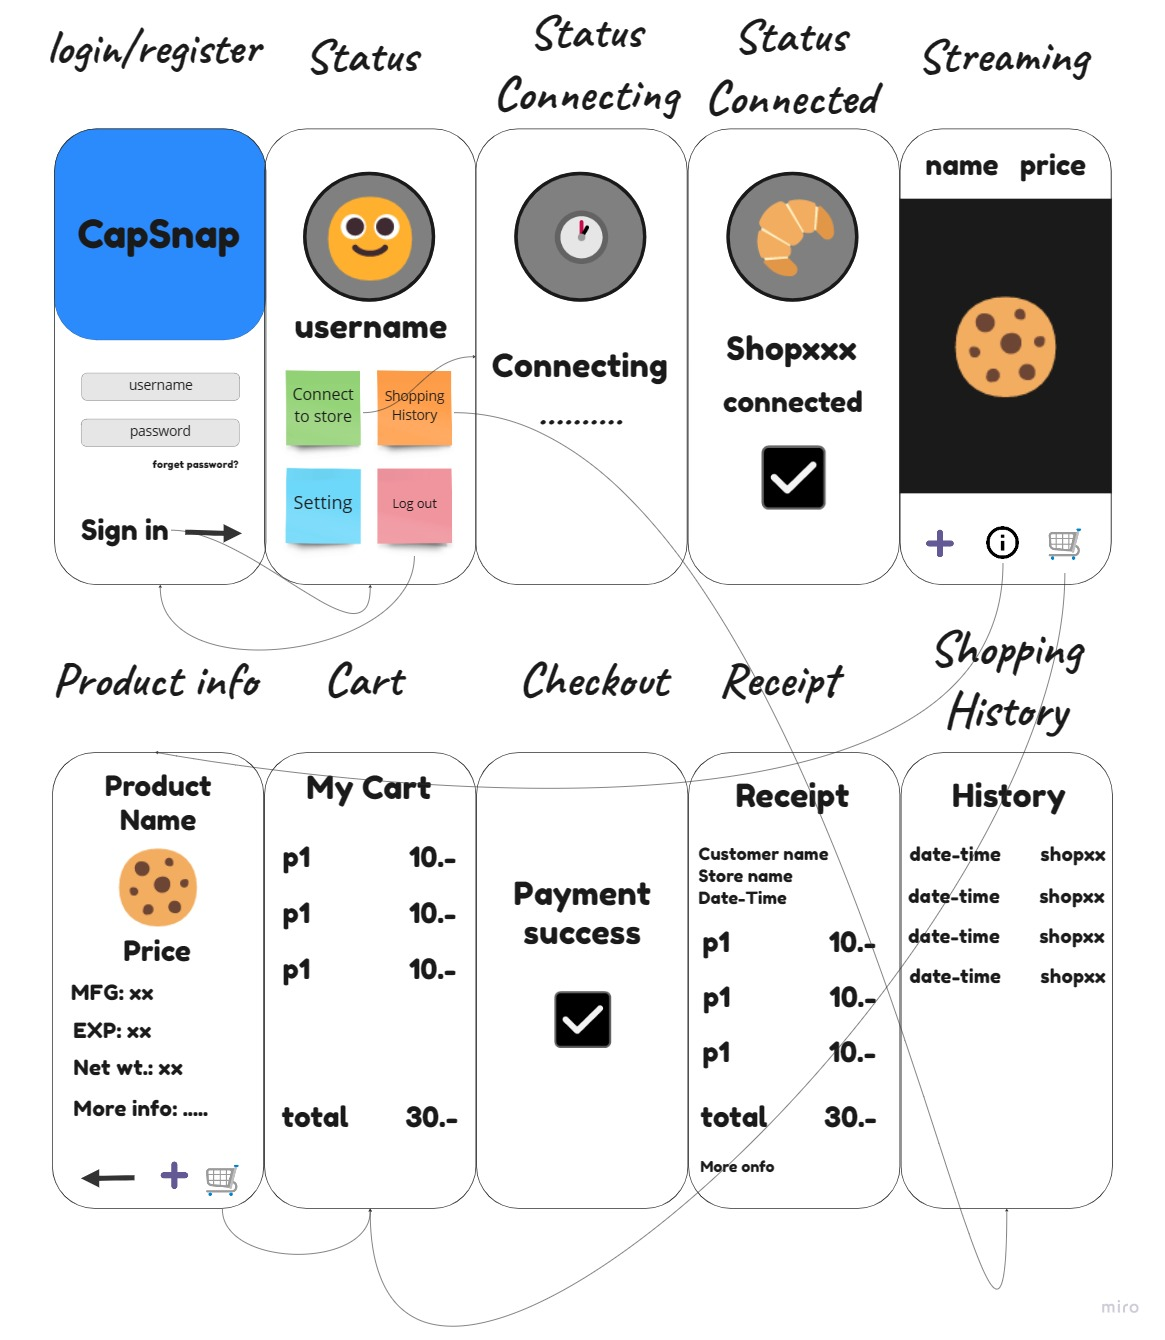
\includegraphics[scale=0.25]{pic/ui/mobileui.jpg}
    \end{center}
    
    \caption[Application wire frame]{Application wire frame}
    \label{fig:Application wire frame}
    \end{figure} 

ในส่วนของการออกแบบส่วนสื่อประสานกับผู้ใช้ (GUI) ของแอพลิเคชันมือถือนั้น ได้กำหนดให้มีหน้าการใช้งานหลักทั้งหมด 10 หน้า ได้แก่
 
    \begin{enumerate}
        \item Login/Register page: หน้าการเข้าสู่ระบบ หรือลงทะเบียนเข้าใช้งาน
        \item Home page: หน้าแสดงชื่อผู้ใช้ และเมนูของฟังก์ชันต่าง ๆ
        \item Connecting page: หน้าการเชื่อมต่อกับร้านค้าซึ่งสามารถแสกนคิวอาร์โค้ดที่ร้านค้าได้เพื่อเข้าสู่หน้าการเลือกซื้อสินค้าหลังเชื่อต่อกับร้านค้าสำเร็จ
        \item Connection status page: แสดงสถานการณ์เชื่อต่อกับร้านค้า
        \item Streaming page: หน้าฟังก์ชันการสตรีมมิ่งรูปภาพสินค้าผ่านกล้องมือถือแบบเรียลไทม์ ซึ่งจะแสดงชื่อ และราคาของสินค้า ซึ่งมีปุ่มการทำงานดังนี้ ปุ่มกดดูรายละเอียดสินค้า ,  ปุ่มเพิ่มสินค้าลงตะกร้า , ปุ่มกดดูสินค้าในตะกร้า
        \item Product information page: หน้าแสดงรายละเอียดของสินค้า
        \item My cart page: หน้าแสดง และจัดการเพิ่ม-ลบสินค้าในตะกร้า
        \item Checkout page: หน้าการชำระเงิน
        \item Receipt page: หน้าแสดงใบเสร็จหลังชำระเงินสำเร็จ
        \item History page: หน้าแสดงประวัติการซื้อสินค้า
    \end{enumerate}
    % 1.	Login/Register page: หน้าการเข้าสู่ระบบ หรือลงทะเบียนเข้าใช้งาน
    % 2.	Home page: หน้าแสดงชื่อผู้ใช้ และเมนูของฟังก์ชันต่าง ๆ
    % 3.	Connecting page: หน้าการเชื่อมต่อกับร้านค้าซึ่งสามารถแสกนคิวอาร์โค้ดที่ร้านค้าได้เพื่อเข้าสู่หน้าการเลือกซื้อสินค้าหลังเชื่อต่อกับร้านค้าสำเร็จ
    % 4.	Connection status page: แสดงสถานการณ์เชื่อต่อกับร้านค้า
    % 5.	Streaming page: หน้าฟังก์ชันการสตรีมมิ่งรูปภาพสินค้าผ่านกล้องมือถือแบบเรียลไทม์ ซึ่งจะแสดงชื่อ และราคาของสินค้า ซึ่งมีปุ่มการทำงานดังนี้
    % a.	ปุ่มกดดูรายละเอียดสินค้า
    % b.	ปุ่มเพิ่มสินค้าลงตะกร้า
    % c.	ปุ่มกดดูสินค้าในตะกร้า
    % 6.	Product information page: หน้าแสดงรายละเอียดของสินค้า
    % 7.	My cart page: หน้าแสดง และจัดการเพิ่ม-ลบสินค้าในตะกร้า
    % 8.	Checkout page: หน้าการชำระเงิน
    % 9.	Receipt page: หน้าแสดงใบเสร็จหลังชำระเงินสำเร็จ
    % 10.	History page: หน้าแสดงประวัติการซื้อสินค้า
    



    \section{Web Dashboard UX/UI}
    % \begin{center}
{
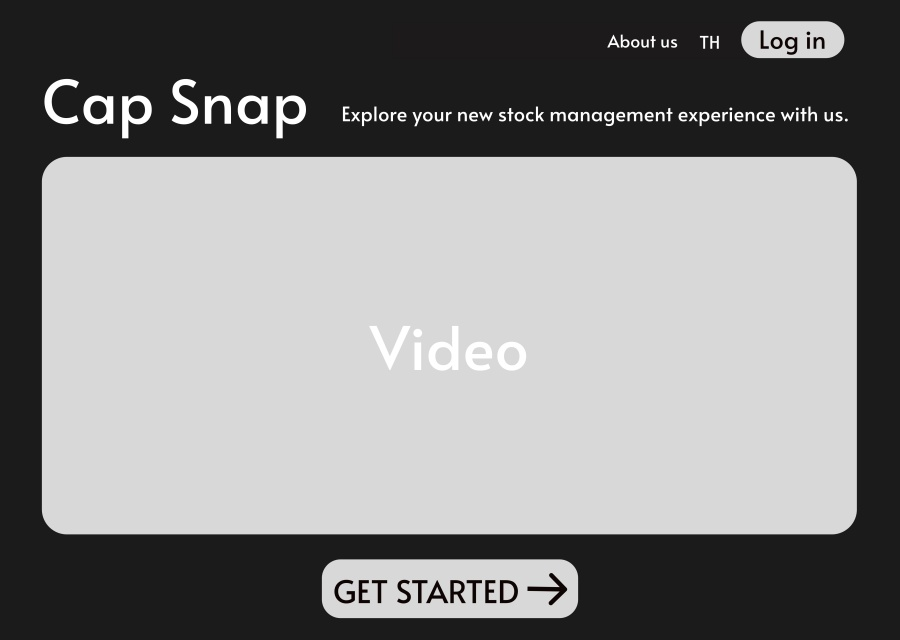
\includegraphics[scale=0.9]{pic/ui/1.jpg}
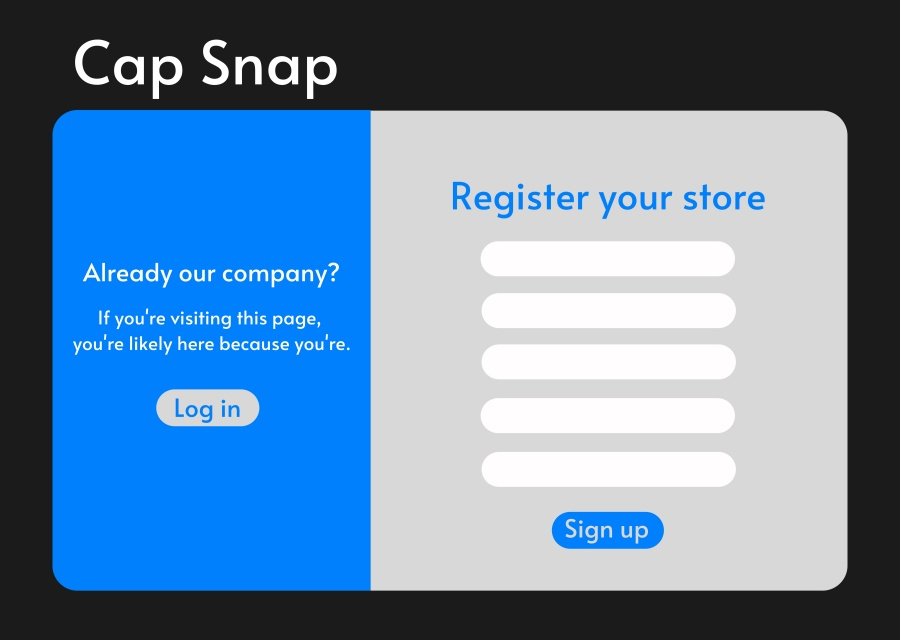
\includegraphics[scale=0.9]{pic/ui/2.jpg}
}\\
{
 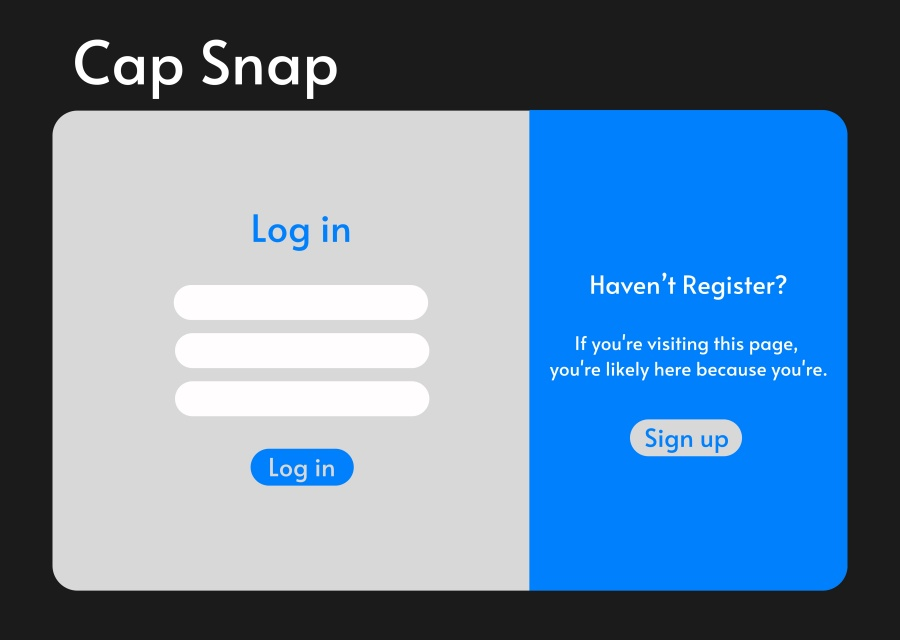
\includegraphics[scale=0.9]{pic/ui/3.jpg}
 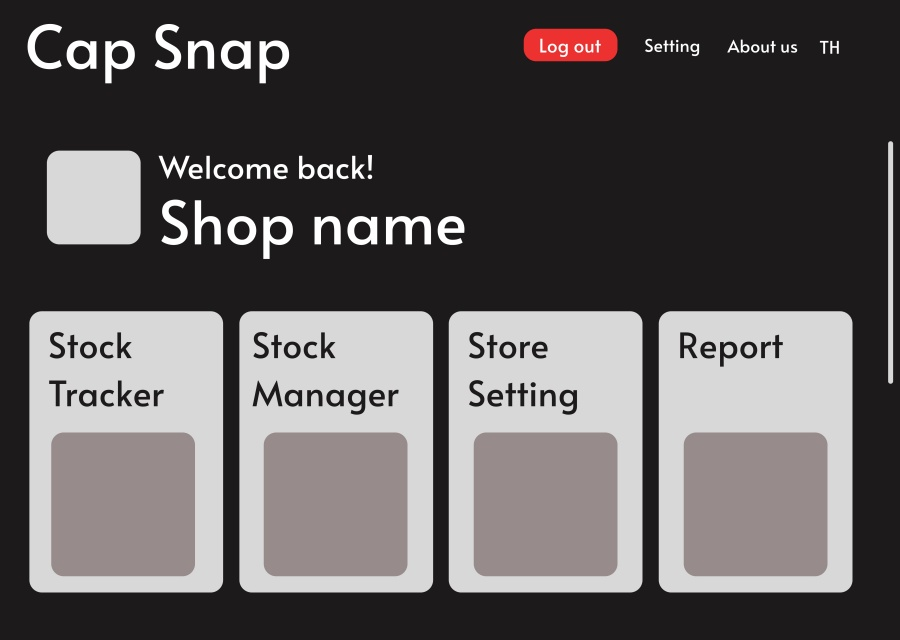
\includegraphics[scale=0.9]{pic/ui/4.jpg}
}\\
{
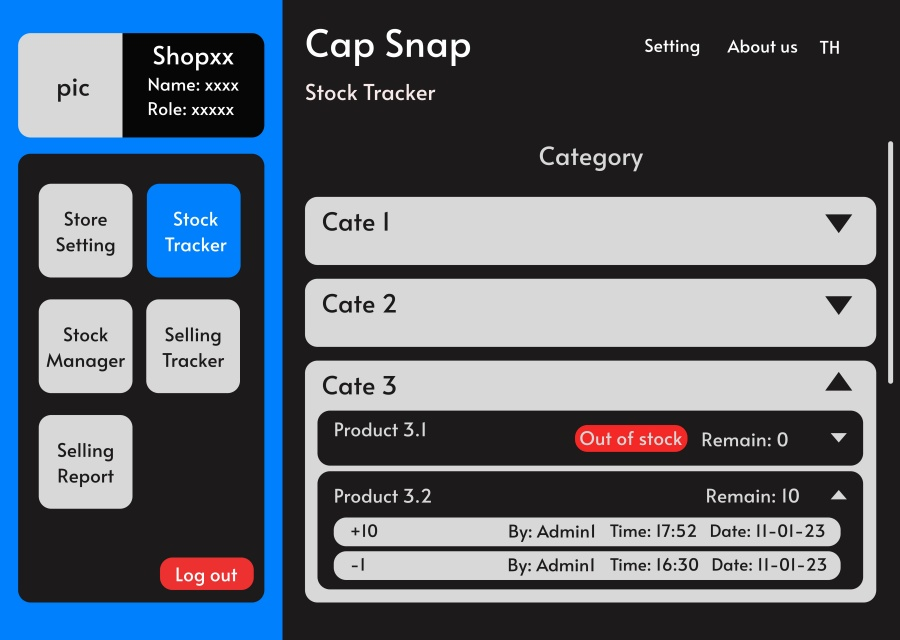
\includegraphics[scale=0.9]{pic/ui/5.jpg}
% 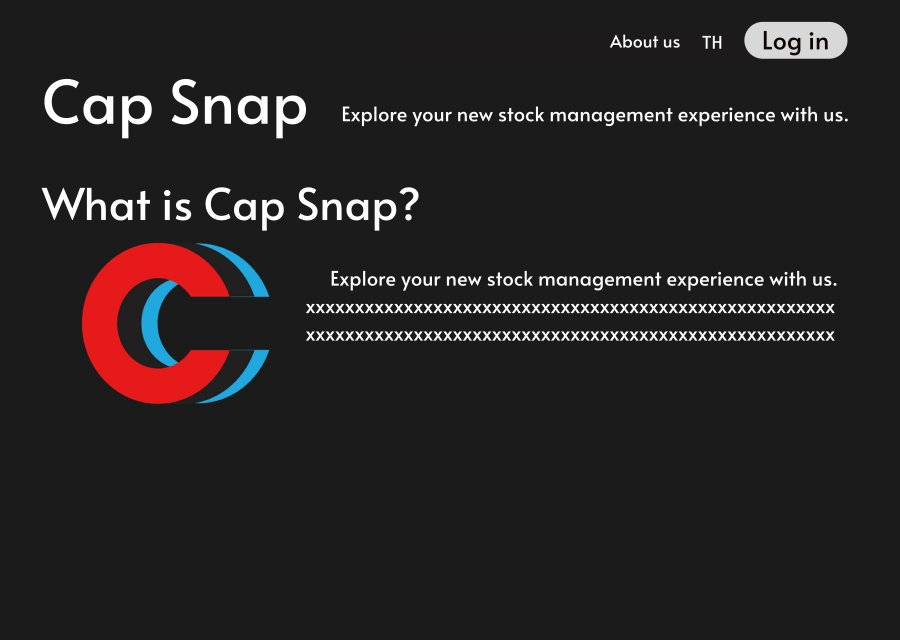
\includegraphics[scale=0.9]{pic/ui/6.jpg}
}\\
{
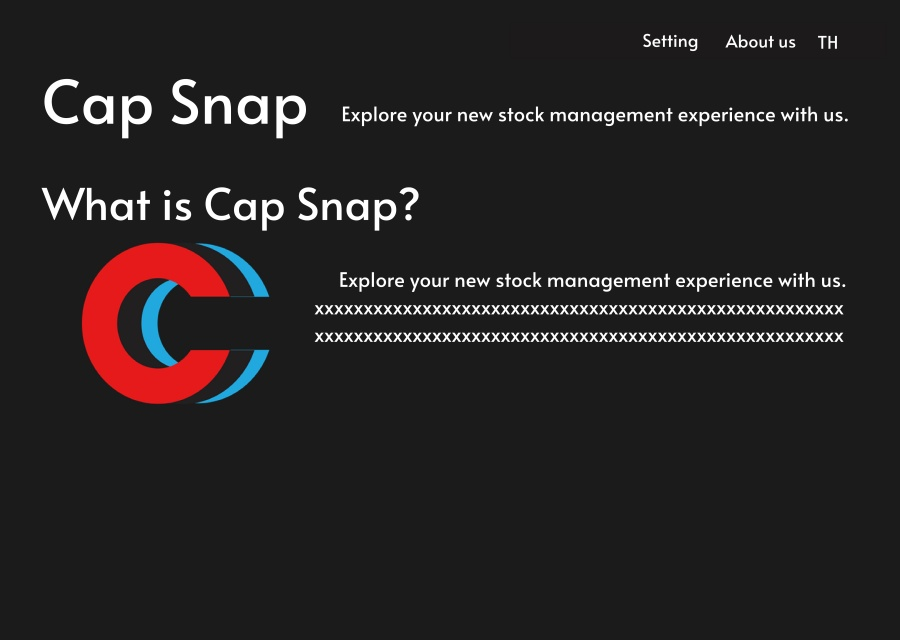
\includegraphics[scale=0.9]{pic/ui/7.jpg}
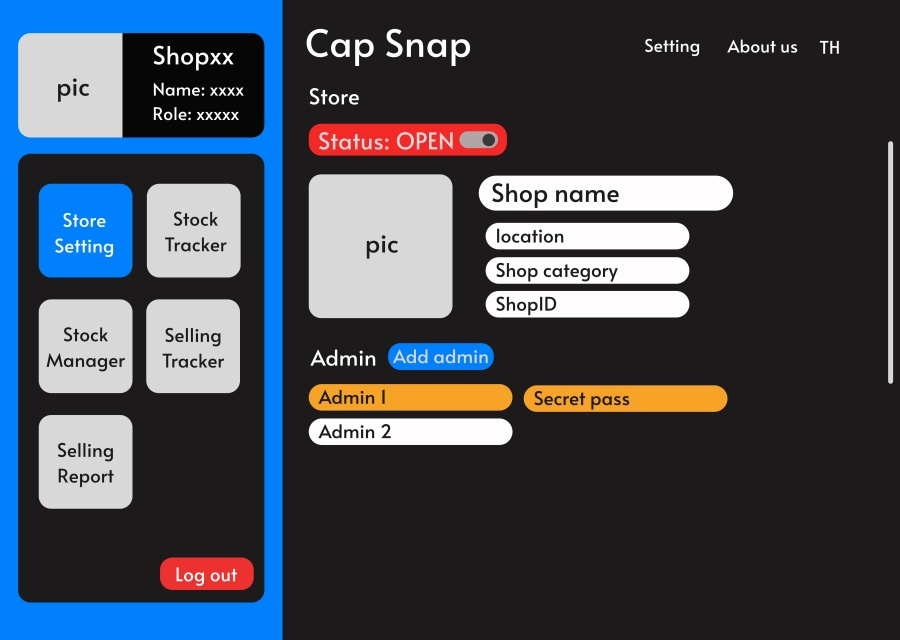
\includegraphics[scale=0.9]{pic/ui/8.jpg}
}\\
{
 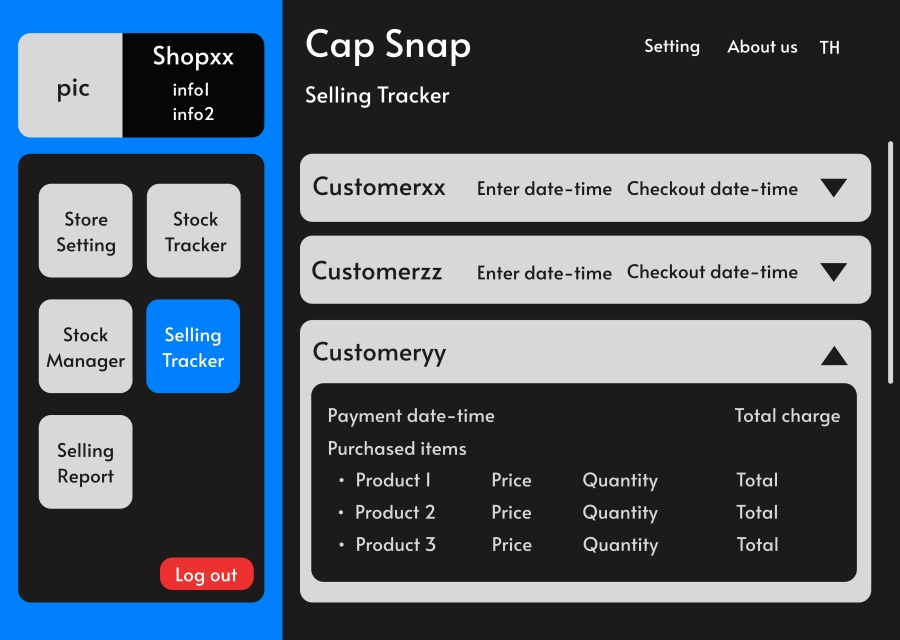
\includegraphics[scale=0.9]{pic/ui/9.jpg}
 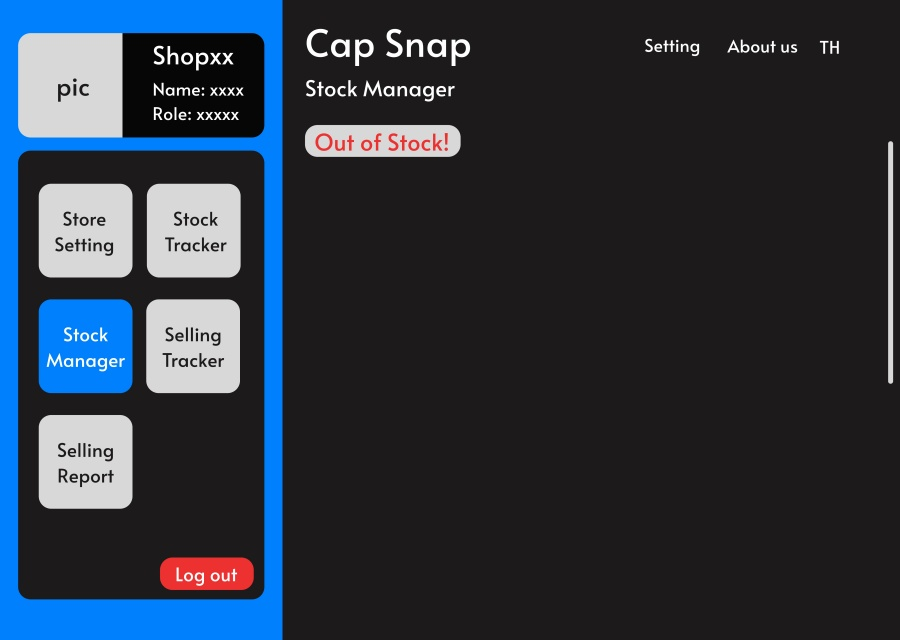
\includegraphics[scale=0.9]{pic/ui/10.jpg}
}\\
{
 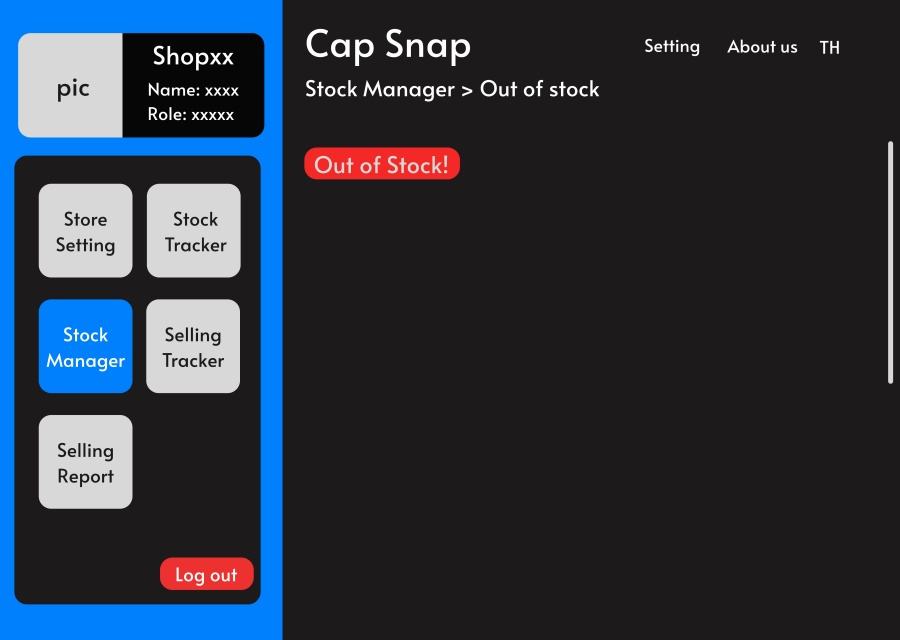
\includegraphics[scale=0.9]{pic/ui/11.jpg}
 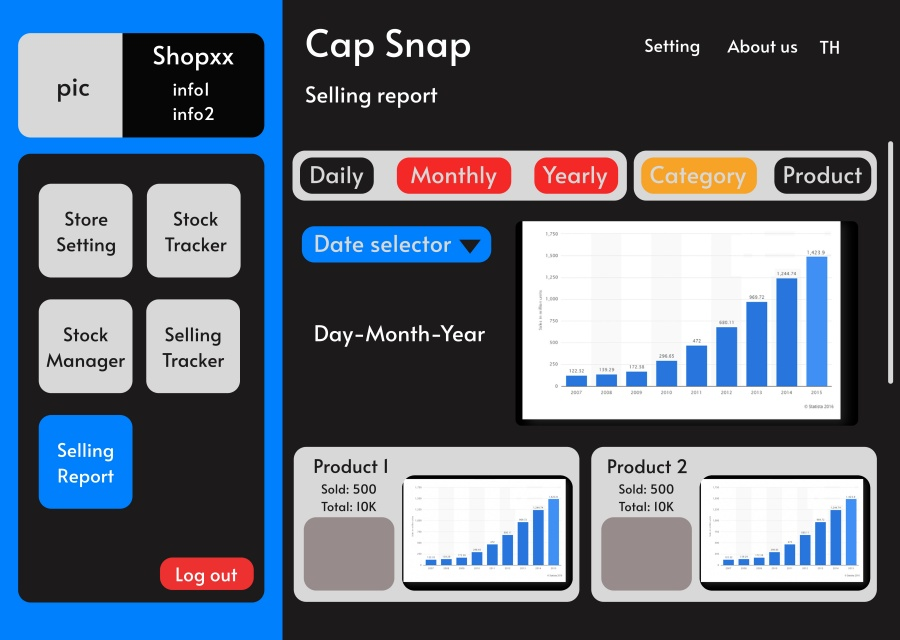
\includegraphics[scale=0.9]{pic/ui/12.jpg}
}


ในส่วนของการออกแบบส่วนสื่อประสานกับผู้ใช้ (GUI) ของ Website Dashboard นั้น ได้กำหนดให้มีหน้าการใช้งานหลักทั้งหมด 11 หน้า ได้แก่
\begin{enumerate}
    \item Get started page: หน้าการเข้าสู่ระบบ หรือลงทะเบียนเข้าใช้งาน
    \item Login page: หน้าการเข้าสู่ระบบ
    \item Register page: หน้าการลงทะเบียนเข้าใช้งาน
    \item Home page:  หน้าแสดงเมนูของฟังก์ชันต่าง ๆ
    \item Store setting page: หน้าการตั้งค่าข้อมูลร้านค้า
    \item Stock tracker page: หน้าการติดตามคลังสินค้า
    \item Stock manager page: หน้าการจัดการคลังสินค้า
    \item Stock manager page > Out of stock page: หน้าการจัดการสินค้าที่ไม่เหลือในคลัง
    \item Selling tracker page: หน้าการติดตามยอดขายตามลำดับคำสั่งซื้อ
    \item Selling report page: หน้าการแสดงผลข้อมูลยอดขายตามรายวัน รายเดือน และรายปี โดยสามารถดูตามหมวดหมู่ของสินค้า หรือแยกตามสินค้าหนึ่ง ๆได้
    \item About us page: หน้าแสดงรายละเอียดของผลิตภัณฑ์ของเรา
\end{enumerate}
 
 
% 1.	Get started page: หน้าการเข้าสู่ระบบ หรือลงทะเบียนเข้าใช้งาน
% 2.	Login page: หน้าการเข้าสู่ระบบ
% 3.	Register page: หน้าการลงทะเบียนเข้าใช้งาน
% 4.	Home page:  หน้าแสดงเมนูของฟังก์ชันต่าง ๆ
% 5.	Store setting page: หน้าการตั้งค่าข้อมูลร้านค้า
% 6.	Stock tracker page: หน้าการติดตามคลังสินค้า
% 7.	Stock manager page: หน้าการจัดการคลังสินค้า
% 8.	Stock manager page > Out of stock page: หน้าการจัดการสินค้าที่ไม่เหลือในคลัง
% 9.	Selling tracker page: หน้าการติดตามยอดขายตามลำดับคำสั่งซื้อ
% 10.	Selling report page: หน้าการแสดงผลข้อมูลยอดขายตามรายวัน รายเดือน และรายปี โดยสามารถดูตามหมวดหมู่ของสินค้า หรือแยกตามสินค้าหนึ่ง ๆได้
% 11.	About us page: หน้าแสดงรายละเอียดของผลิตภัณฑ์ของเรา

    
    % \end{center}

